\documentclass{article}[12pt]
\usepackage{color}
\usepackage[normalem]{ulem}
\usepackage{times}
\usepackage{fullpage}
\usepackage{amsmath}
\usepackage{amssymb}
\usepackage{tikz}
\def \R {\mathbb R}
\def \imp {\Longrightarrow}
\def \eps {\varepsilon}
\def \Inf {{\sf Inf}}
\newenvironment{proof}{{\bf Proof.  }}{\hfill$\Box$}
\newtheorem{theorem}{Theorem}[section]
\newtheorem{definition}{Definition}[section]
\newtheorem{corollary}{Corollary}[section]
\newtheorem{lemma}{Lemma}[section]
\newtheorem{claim}{Claim}[section]
\setlength {\parskip}{2pt}
\setlength{\parindent}{0pt}

\newcommand{\headings}[4]{\noindent {\bf Assignment 10 CME241} \hfill {{\bf Author:} Nicolas Sanchez} \\
{} \hfill {{\bf Due Date:} #2} \\

\rule[0.1in]{\textwidth}{0.025in}
}

\newcommand{\klnote}[1]{{\color{red} #1}}
\newcommand{\klsout}[1]{{\color{red} \sout{#1}}}

\begin{document}

\headings{\#1}{Tuesday, October 8, 10:30am}\section{} 



\section{Optimal Market Making Special Cases}
We consider the special case:
$$ V(t,S_t, W, I) = E[-e^{-\gamma(W+I\cdot S_T)}| t,S_t] = -e^{-\gamma W} E[e^{-\gamma I \cdot S_T} | t, S_t]$$
where we have $S_{t_2} \sim \mathbf{N}(S_{t_1}, \sigma^2(t_2 - t_1))$ and therefore $-\gamma I \cdot S_T \sim \mathbf{N}(-\gamma I \cdot S_t, \gamma I \sigma^2(T-t))$ which yields using the expectation of a lognormal variable:
$$ V(t,S_t, W, I) =  -e^{-\gamma W} e^{-\gamma I \cdot S_t + \frac{1}{2}\gamma I \sigma^2(T-t)} = -e^{-\gamma(W+I(S_t-\frac{\sigma^2(T-t)}{2}))}$$
Now denote $Q^{(b)}(t,S_t, I) = q_b$ and $Q^{(a)}(t,S_t, I) = q_a$ so we compute:
\begin{align*}
V(t, S_t, W - q_b, I+1) &= V(t, S_t, W, I)\\
-e^{-\gamma(W-q_b+(I+1)(S_t-\frac{\sigma^2(T-t)}{2}))} &= -e^{-\gamma(W+I(S_t-\frac{\sigma^2(T-t)}{2}))}\\
-\gamma(W-q_b+(I+1)(S_t-\frac{\sigma^2(T-t)}{2})) &= -\gamma(W+I(S_t-\frac{\sigma^2(T-t)}{2}))\\
-q_b+S_t-\frac{\sigma^2(T-t)}{2}) &=0\\
q_b &= S_t-\frac{\sigma^2(T-t)}{2}\\
\end{align*}

We do the same for $q_a$:
\begin{align*}
V(t, S_t, W + q_a, I-1) &= V(t, S_t, W, I)\\
-e^{-\gamma(W+q_a+(I-1)(S_t-\frac{\sigma^2(T-t)}{2}))} &= -e^{-\gamma(W+I(S_t-\frac{\sigma^2(T-t)}{2}))}\\
-\gamma(W+q_a+(I-1)(S_t-\frac{\sigma^2(T-t)}{2})) &= -\gamma(W+I(S_t-\frac{\sigma^2(T-t)}{2}))\\
q_a-(S_t-\frac{\sigma^2(T-t)}{2}) &=0\\
q_a&= S_t-\frac{\sigma^2(T-t)}{2}\\
\end{align*}

Hence indifferent bid and offer are both $\frac{\sigma^2(T-t)}{2}$ from the mid price at times $S_t$.
\section{Optimal Performance Policy Test}
We implement the suggested strategy in test\_optimal\_mm.py and do indeed find that the its is a superior strategy - though returns are slightly lower the variance is significantly decreased for the AS optimal strategy as seen below.

\begin{figure}
  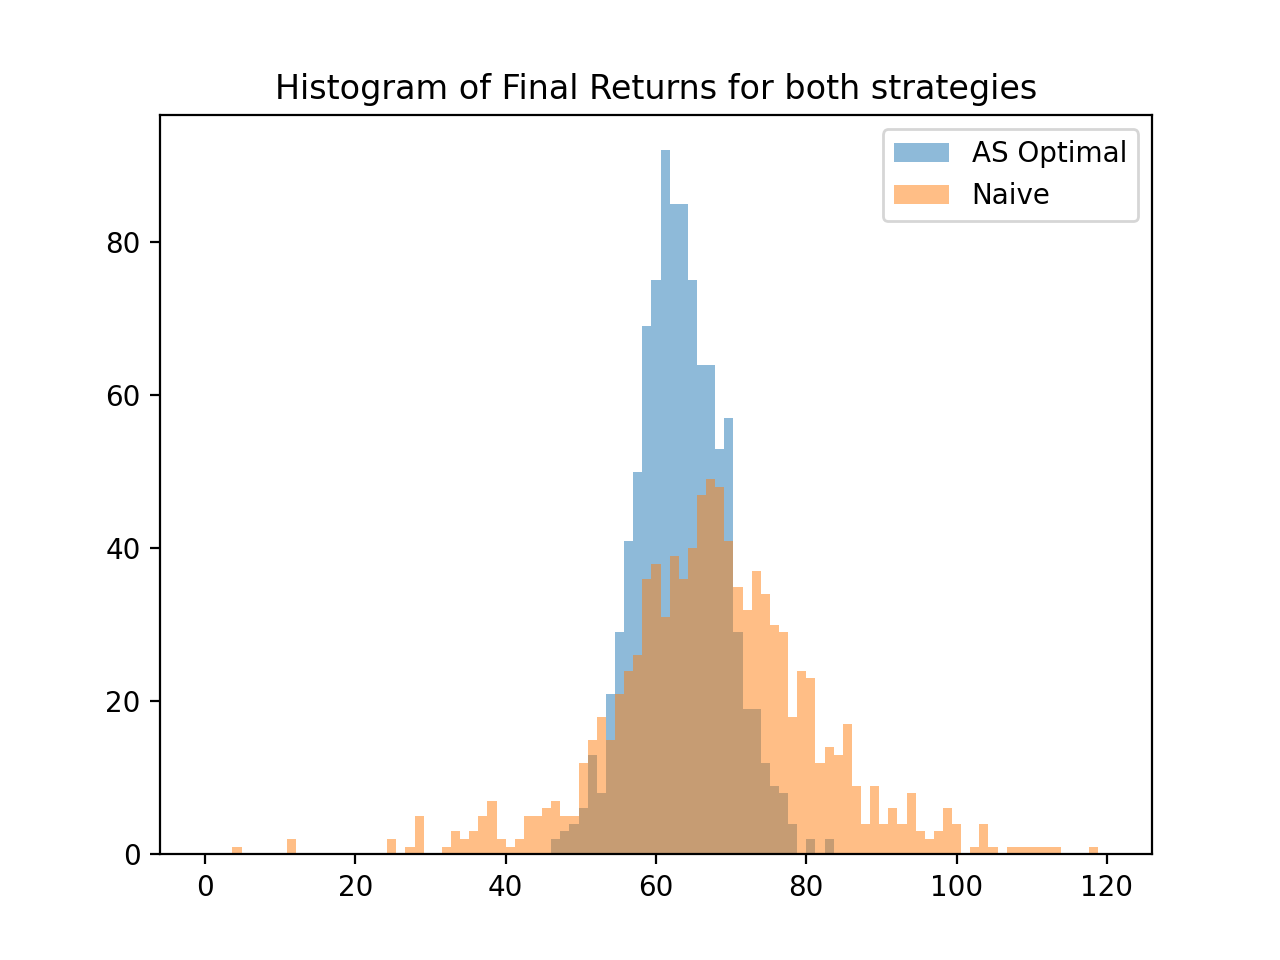
\includegraphics[width=\linewidth]{histogram.png}
  \caption{Allocation with varying alphas}
  \label{fig:llp3}
\end{figure}
\end{document}
